%----------------------------------------------------------------------------------------
% PACKAGES AND OTHER DOCUMENT CONFIGURATIONS
%----------------------------------------------------------------------------------------

\documentclass[9pt]{./src/packages/Developer_CV/developercv}
\usepackage{amssymb}
\usepackage{fontawesome}
\usepackage{enumitem}
\usepackage{ifpdf}
\graphicspath{ {./img/} }

\begin{document}

%----------------------------------------------------------------------------------------
% PHOTO, NAME, CONTACT
%----------------------------------------------------------------------------------------

\begin{minipage}[t]{0.15\textwidth} % 30% of the page width for photo
    \vspace{-\baselineskip} % Required for vertically aligning minipages
    \raggedright % Align to left as possible
    \setlength{\fboxsep}{0pt} % Removes the gap between the image and the border
    \setlength{\fboxrule}{3pt} % Add border
    \ifpdf
        \fbox{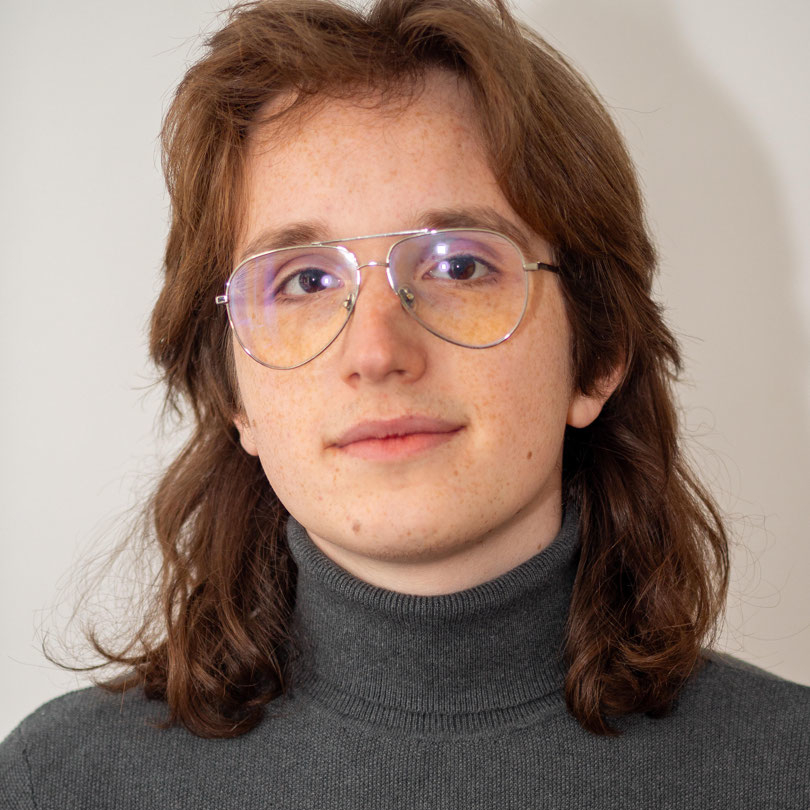
\includegraphics[width=\linewidth]{./src/img/photo_square.jpg}}
    \else
        \fbox{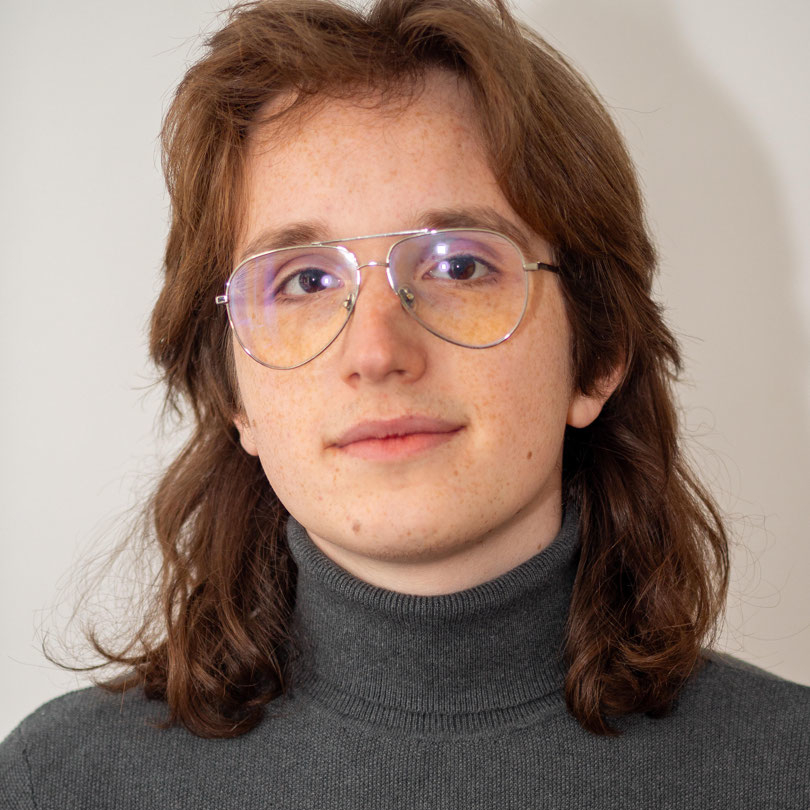
\includegraphics[width=\linewidth,natwidth=810,natheight=810]{./src/img/photo_square.jpg}}
    \fi
\end{minipage}
\hspace{1.5pt} % Adjust this to remove space caused by the fbox
\begin{minipage}[t]{0.49\textwidth} % 45% of the page width for name
    \vspace{-\baselineskip} % Required for vertically aligning minipages
    \colorbox{black}{{\HUGE\textcolor{white}{\textbf{\MakeUppercase{Tymoteusz}}}}} % First name

    \colorbox{black}{{\HUGE\textcolor{white}{\textbf{\MakeUppercase{Burak}}}}} % Last name

    \vspace{6pt}

    \hspace{1.5pt} % Adjust this to align with top text
    {\huge Embedded Systems Engineer} % Career or current job title

\end{minipage}
\begin{minipage}[t]{0.35\textwidth} % 35% of the page width for the first row of icons
    %\vspace{-\baselineskip} % Required for vertically aligning minipages
    \raggedright % Align to left as possible

    % START SUBSTITUTE
    \icon{MapMarker}{8}{\rule{10em}{1em}}\\
    \icon{Phone}{8}{+\rule{2em}{1em} \rule{9em}{1em}}\\
    % END SUBSTITUTE
    \icon{At}{8}{\href{mailto:tymbur@gmail.com}{tymbur@gmail.com}}\\
    \icon{Github}{8}{\href{https://github.com/tym2k1}{github.com/tym2k1}}\\
    \icon{Linkedin}{8}{\href{https://www.linkedin.com/in/tymoteusz-burak/}{linkedin.com/in/tymoteusz-burak}}\\

\end{minipage}
\\

%----------------------------------------------------------------------------------------
% INTRODUCTION, SKILLS AND TECHNOLOGIES
%----------------------------------------------------------------------------------------

\vspace{-0.3cm} % move the "who am i?" section up
\noindent % Prevents indentation
\begin{minipage}[t]{0.60\textwidth} % 45% of the page width for the introduction text
    \cvsect{Who Am I?}
    \raggedright

    A low-level enthusiast with a strong drive for engineering,
    innovation, and problem-solving. I am pursuing a career in research and
    development (R\&D), with a focus on critical embedded systems.

    I love hard problems, working in a team, and keeping things relaxed.
    I especially enjoy spaces where I can dive deep into creative technical work
    with a team like in hackathons.

    Beyond engineering, I’m drawn to experimental, math-driven art, occasionally
    exploring algorithmic approaches to music and design, when time allows.

\end{minipage}
\hfill % Horizontal space between the minipages
\begin{minipage}[t]{0.35\textwidth}
    \cvsect{Technologies}
    \raggedright % Align to left as possible
    \\
    \colorbox{black}{\textcolor{white}{\raisebox{0.5ex}[10pt][0pt]{\textbf{Linux}}}}
    \colorbox{black}{\textcolor{white}{\raisebox{0.5ex}[10pt][0pt]{\textbf{Shell Scripting}}}}
    \colorbox{black}{\textcolor{white}{\raisebox{0.5ex}[10pt][0pt]{\textbf{Git}}}}
    \colorbox{black}{\textcolor{white}{\raisebox{0.5ex}[10pt][0pt]{\textbf{Yocto}}}}
    \colorbox{black}{\textcolor{white}{\raisebox{0.5ex}[10pt][0pt]{\textbf{Python}}}}
    \colorbox{black}{\textcolor{white}{\raisebox{0.5ex}[10pt][0pt]{\textbf{Docker}}}}
    \colorbox{black}{\textcolor{white}{\raisebox{0.5ex}[10pt][0pt]{\textbf{Nix}}}}
    \colorbox{black}{\textcolor{white}{\raisebox{0.5ex}[10pt][0pt]{\textbf{Zephyr}}}}
    \colorbox{black}{\textcolor{white}{\raisebox{0.5ex}[10pt][0pt]{\textbf{C}}}}
    \colorbox{black}{\textcolor{white}{\raisebox{0.5ex}[10pt][0pt]{\textbf{CI/CD (Github/Gitea Actions)}}}}
    \colorbox{black}{\textcolor{white}{\raisebox{0.5ex}[10pt][0pt]{\textbf{C++}}}}
    \colorbox{black}{\textcolor{white}{\raisebox{0.5ex}[10pt][0pt]{\textbf{Buildroot}}}}
    \colorbox{black}{\textcolor{white}{\raisebox{0.5ex}[10pt][0pt]{\textbf{Confidential Computing}}}}
    \colorbox{black}{\textcolor{white}{\raisebox{0.5ex}[10pt][0pt]{\textbf{MATLAB}}}}
    \colorbox{black}{\textcolor{white}{\raisebox{0.5ex}[10pt][0pt]{\textbf{LabVIEW}}}}
    \colorbox{black}{\textcolor{white}{\raisebox{0.5ex}[10pt][0pt]{\textbf{LaTeX}}}}
    \\
\end{minipage}

%----------------------------------------------------------------------------------------
% EDUCATION
%----------------------------------------------------------------------------------------

\cvsect{Education}

\begin{entrylist}
    \entry
        {2025 -- Present}
        {Master of Science in Aerospace Informatics}
        {Julius-Maximilians-Universität Würzburg, Germany}
        {
        }
    \entry
        {2020 -- 2024}
        {Bachelor of Engineering in Automation, Robotics and Control Systems}
        {Gdańsk University of Technology, Poland}
        {
        Thesis:\\[0.1em]
        \textit{
        Intelligent system for the analysis of a human skeletal model
        in 3D space to support medical diagnosis, rehabilitation and physical
        activity.}
        }
\end{entrylist}

%----------------------------------------------------------------------------------------
% EXPERIENCE
%----------------------------------------------------------------------------------------

\cvsect{Experience}

\begin{entrylist}
    \raggedright % Align to left as possible
    \entry
    {02/2025--Present}
    {Research Assistant}
    {Chair of Software Engineering - \href{https://se.informatik.uni-wuerzburg.de/en/secure-software-systems-group/}{Secure Software Systems Group}, University of Würzburg, Germany}
    {
        Joined the \href{https://se.informatik.uni-wuerzburg.de/en/secure-software-systems-group/}{Secure Software Systems Group} as a salaried Research Assistant (TV-L), while pursuing my Master’s degree, continuing technical contributions to the \href{https://crosscon.eu/}{CROSSCON Project (Cross-platform Open Security Stack for Connected Devices)} following my prior industry work on the same initiative. The role entails greater responsibility and duties beyond those of student assistants (HiWis).
    \begin{enumerate}
        \item[$\blacksquare$] Contributing to technical deliverables of the \href{https://crosscon.eu/}{CROSSCON Project}.
    \begin{enumerate}
    \item[$\blacksquare$] Implemented a Zero-Knowledge PUF-based authentication trusted service on a static-partitioning hypervisor (Bao/CROSSCON Hypervisor) for Arm Cortex-M (LPC55S69), using Zephyr RTOS as isolated "VMs". Built upon prior cryptographic design to deliver a working proof-of-concept demonstrating potential GlobalPlatform compliance for this architecture.
    \end{enumerate}
        \item[$\blacksquare$] Collaborating with student assistants (HiWis), delegating tasks, conducting code reviews, and providing guidance in embedded systems development and software engineering best practices.
        \item[$\blacksquare$] Supervising cybersecurity-related seminar topics.
    \end{enumerate}
    }
    \entry
    {06/2023--02/2025}
    {Junior Embedded Systems Engineer}
    {3mdeb Sp. z o. o., Gdańsk, Poland}
    {
    Worked on the Embedded Systems team with a focus on Linux firmware development for hardened secure targets and implementing emerging technologies such as FIDO Device Onboarding, fTPM, Measured Boot, and secure OTA updates.
    \begin{enumerate}
        \item[$\blacksquare$] Developed custom Linux distributions using Yocto, Buildroot, and OpenWRT, including work on the \href{https://docs.zarhus.com/}{Zarhus OS}.
        \begin{enumerate}
            \item[$\blacksquare$] Worked on board support packages and device tree configurations for embedded targets.
            \item[$\blacksquare$] Developed test cases, CI/CD pipelines and documentation.
            \item[$\blacksquare$] Contributed patches and improvements to upstream open-source projects as part of integration efforts.
        \end{enumerate}
        \item[$\blacksquare$] Contributed to the \href{https://crosscon.eu/}{CROSSCON Project (Cross-platform Open Security Stack for Connected Devices)}:
        \begin{enumerate}
            \item[$\blacksquare$] Co-developed validation criteria and high-level architecture for embedded security use-cases.
            \item[$\blacksquare$] Participated in implementation planning, prototyping, and reporting on project milestones.
            \item[$\blacksquare$] Authored blog post: \href{https://crosscon.eu/blog/embracing-ftpm-embedded-arm-devices-insights-and-solutions}{\textit{Embracing fTPM on Embedded ARM Devices}}.
        \end{enumerate}
        \item[$\blacksquare$] Public speaking:
        \begin{enumerate}
            \item[$\blacksquare$] \textbf{Yocto Project Developer Day 2024} (Co-Speaker): {\href{https://www.youtube.com/watch?v=W78AKeWh57g}{\textit{Practical Security for Embedded Systems: Implementing TEE and Secure Storage}}}.
            \item[$\blacksquare$] \textbf{Dasharo Developer vPub \#6}: {\href{https://www.youtube.com/watch?v=9vBZeIZnS3o}{\textit{Dasharo Configuration Utility - Status Update}}}.
            \item[$\blacksquare$] \textbf{FOSDEM 2024}: {\href{https://archive.fosdem.org/2024/schedule/event/fosdem-2024-3097-securing-embedded-systems-with-ftpm-implemented-as-trusted-application-in-tee/}{\textit{Securing Embedded Systems with fTPM implemented as Trusted Application in TEE}}}.
            \item[$\blacksquare$] \textbf{Yocto Summit 2023}: {\href{https://www.youtube.com/watch?v=Wg1ZUdwTYNM&t=1s}{\textit{FIDO Device Onboarding: Late-binding Provisioning \& Tales from the Trenches of Bleeding Edge Tech}}}.
        \end{enumerate}
    \end{enumerate}
    }
    \entry
        {03/2021--11/2021}
        {Technical Support and Junior Vision Systems Engineer}
        {VisionX, Gdańsk, Poland}
        {
        I initially provided general technical support and later transitioned into prototyping industrial vision systems.
        \begin{enumerate}
            \item[$\blacksquare$] Managed a local server running on Windows Server 2019 for remote device access.
            \item[$\blacksquare$] Prototyped/Developed industrial vision systems in LabVIEW / NI Vision:
            \begin{enumerate}
                \item[$\blacksquare$] LED lamp covers burn mark detection.
                \item[$\blacksquare$] Onion rotation detection for food manufacturing.
                \item[$\blacksquare$] Software blueprint for PCB inspections.
            \end{enumerate}
            \item[$\blacksquare$] Collaborated on the development of a QR/Datamatrix code scanner using an STM32-based platform.
        \end{enumerate}
        }
    \end{entrylist}

\cvsect{Volunteering \& Clubs}
\begin{entrylist}
    \entry
        {07/2025--Present}
        {Member - WüSpace e.V.}
        {Würzburg, Germany}
        {
            Participating in the open-lab environment. Onboarding into projects related to aerospace engineering. (In progress) \\
        }
    \entry
        {06/2024--Present}
        {Member - Hackerspace Pomerania}
        {Gdańsk, Poland}
        {
            Contributed to ad hoc prototyping and electronics experiments in a collaborative open-lab environment. \\
        }
    \entry
        {05/2021--06/2023}
        {Member - SimLE Science Club}
        {Gdańsk, Poland}
        {
            Participated in the Science Club’s \href{https://simle.pl/en/projekty/silverhand/}{"Silverhand"} project, contributing to the second iteration of a prosthetic hand,, and later moved on to the \href{https://simle.pl/en/projekty/simba/}{"SimBa"} sounding rocket project, working within the ground segment team.
        \begin{enumerate}
            \item[$\blacksquare$] Collaborated on a prosthetic hand firmware using an STM32-based platform.
            \item[$\blacksquare$] Worked on designing and implementing the backend for a ground control module of a sounding rocket, using Python, InfluxDB, and Mavlink.
            \item[$\blacksquare$] Prototyped an automated motorized radio antenna and camera mount for rocket tracking, leveraging Python and OpenCV.
        \end{enumerate}
        }
    \end{entrylist}
%----------------------------------------------------------------------------------------
% ADDITIONAL INFORMATION
%----------------------------------------------------------------------------------------

\vfill

\begin{minipage}[t]{0.5\textwidth}
    \cvsect{Languages}
    \\
    \textbf{Polish}\\Native\\ \\
    \textbf{English}\\Full Professional Proficiency \\
    \textit{ACERT C1 Academic Certificate}
\end{minipage}
\hfill
\begin{minipage}[t]{0.5\textwidth}
    \cvsect{Interests}
    \raggedright % Align to left as possible
    \\
    \colorbox{black}{\textcolor{white}{\raisebox{0.5ex}[10pt][0pt]{\textbf{Music}}}}
    \colorbox{black}{\textcolor{white}{\raisebox{0.5ex}[10pt][0pt]{\textbf{Art}}}}
    \colorbox{black}{\textcolor{white}{\raisebox{0.5ex}[10pt][0pt]{\textbf{FOSS}}}}
    \colorbox{black}{\textcolor{white}{\raisebox{0.5ex}[10pt][0pt]{\textbf{Cybersecurity}}}}
    \colorbox{black}{\textcolor{white}{\raisebox{0.5ex}[10pt][0pt]{\textbf{Control Theory}}}}
    \colorbox{black}{\textcolor{white}{\raisebox{0.5ex}[10pt][0pt]{\textbf{Making}}}}
    \colorbox{black}{\textcolor{white}{\raisebox{0.5ex}[10pt][0pt]{\textbf{Hacking}}}}
    \colorbox{black}{\textcolor{white}{\raisebox{0.5ex}[10pt][0pt]{\textbf{Tinkering}}}}
\end{minipage}

%----------------------------------------------------------------------------------------

% \vfill
% \centering
% \scriptsize
% Wyrażam zgodę na przetwarzanie moich danych osobowych dla potrzeb niezbędnych do realizacji procesu rekrutacji (zgodnie z ustawą z dnia 10 maja 2018 roku o ochronie danych osobowych (Dz. Ustaw z 2018, poz. 1000) oraz zgodnie z Rozporządzeniem Parlamentu Europejskiego i Rady (UE) 2016/679 z dnia 27 kwietnia 2016 r. w sprawie ochrony osób fizycznych w związku z przetwarzaniem danych osobowych i w sprawie swobodnego przepływu takich danych oraz uchylenia dyrektywy 95/46/WE (RODO).

\end{document}
